\noindent{1.扫描给定的源程序,累计在每个源程序中 C 语言关键字出现的频度
	(为保证查找效率,建议自建哈希表的平均查找长度不大于2),
	通过这种方式扫描两个源程序,提取其特征向量。}

\noindent{2.通过计算向量Xi和Xj的相似值来判断对应两个程序的相似性,
相似值的判别函数计算公式为:}
\begin{equation}
	S(X_i,X_j)=\frac{X_i^T\cdot X_j}{|X_i|\cdot|X_j|}\label{eq:equation}
\end{equation}
\noindent{\;\;\,\ 通过这种方式,可以初步判断两个源程序的相似性,
如图1所示。其中 S 反映了两向量的夹角的余弦,当 S 趋近于 1 时,
两向量夹角趋于 0 ,即两向量趋于相似,反之亦然。}
\begin{figure}[htbp]
	\centering
	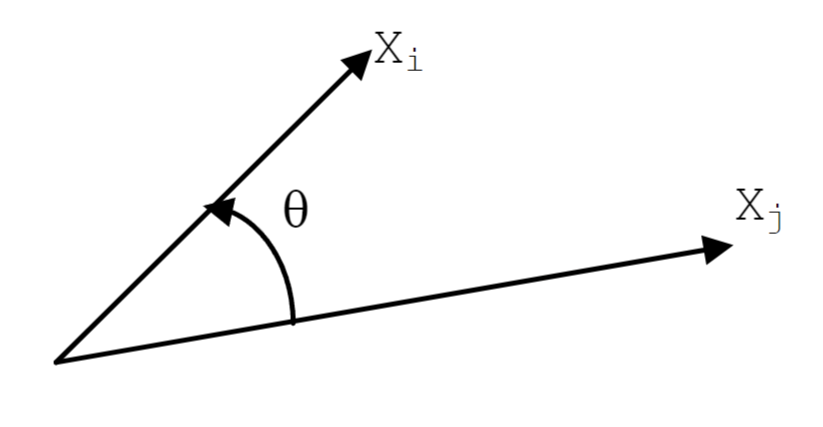
\includegraphics[height=120pt]{S}
	\caption{Similarity}
\end{figure}

\noindent{3.在有些情况下,S 不能很好地反映两向量的相似性,还需要进一步的考虑。
例如,在 S 接近于 1 时,两向量的模的差距不能很好地被反映,如图2所示。
因此引入几何距离 D ,用于反应两向量终点间的距离。}
\begin{figure}[htbp]
	\centering
	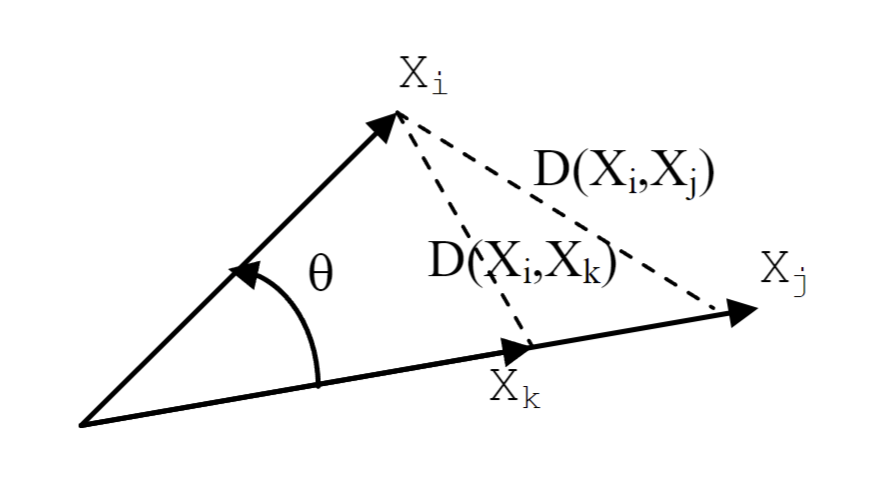
\includegraphics[height=120pt]{D}
	\caption{Distance}
\end{figure}

\noindent{4.通过分别比较很相近和差别很大的三个源代码,实践这种方法的有效性。}
